\documentclass{beamer}

\usepackage[english]{babel}
\usepackage{beamerthemeBoadilla}
%\usepackage{beamerthemeCambridgeUS}
%\usepackage{beamerthemeRochester}
%\usepackage{beamerthemeSzeged}
%\usepackage{beamerthemeMontpellier}
%\usepackage{beamerthemedefault}
\usepackage{url}
\usepackage{verbatim}
\usepackage[utf8]{inputenc}
\usepackage{multirow}
\usepackage{fancyvrb}
\usepackage{proof-dashed}
\newcommand{\mz}{\m{match} \;}
\newcommand{\stepz}{\m{step} \;}
\newcommand{\tab}[0]{\;\;\;\;}
\newcommand{\dz}{\m{derive}~}
\newcommand{\comp}[0]{\m{comp} \;}
\newcommand{\az}{\m{apply} \;}
\newcommand{\doz}{\m{run} \;}
\newcommand{\seqnocut}[3]{#1 ; #2 \Rightarrow #3}
\newcommand{\defeq}{\buildrel\triangle\over =}
\newcommand{\compr}[1]{\m{def} \; #1}

\newcommand{\stepo}{\m{step}_{LLD} \;}
\newcommand{\mo}{\m{match}_{LLD} \;}
\newcommand{\contlld}{\m{cont}_{LLD}}
\newcommand{\cont}{\contlld \;}
\newcommand{\contclld}{\m{cont}_{LLDc}}
\newcommand{\contc}{\contclld \;}
\newcommand{\done}{\m{derive}_{LLD} \;}
\newcommand{\doo}{\m{run}_{LLD} \;}
\newcommand{\matchlldc}{\m{match}_{LLDc}}
\newcommand{\mc}[0]{\matchlldc \; }
\newcommand{\dall}[0]{\m{fix}_{LLD} \; }
\newcommand{\strans}[0]{\m{update}_{LLD} \;}
\newcommand{\dc}{\m{derive}_{LLDc} \;}
\newcommand{\ao}{\m{apply}_{LLD} \;}

\newcommand{\com}{\xrightarrow{*}}
%\mapsto}
\newcommand{\feq}[2]{#1 \equiv #2}
\usepackage{latexsym}
\usepackage{amssymb}            % for \multimap (-o)
\usepackage{stmaryrd}           % for \binampersand (&), \bindnasrepma (\paar)

\newcommand{\m}[1]{\mathsf{#1}}
\newcommand{\f}[1]{\framebox{#1}}

\newcommand{\eph}{\mathit{eph}}
\newcommand{\pers}{\mathit{pers}}
\newcommand{\um}[1]{\underline{\m{#1}}}

\newcommand{\seq}{\vdash}
\newcommand{\semi}{\mathrel{;}}
\newcommand{\lequiv}{\mathrel{\dashv\vdash}}

% symbols of linear logic
\newcommand{\lolli}{\multimap}
\newcommand{\tensor}{\otimes}
\newcommand{\with}{\mathbin{\binampersand}}
\newcommand{\paar}{\mathbin{\bindnasrepma}}
\newcommand{\one}{\mathbf{1}}
\newcommand{\zero}{\mathbf{0}}
\newcommand{\bang}{{!}}
\newcommand{\whynot}{{?}}
\newcommand{\bilolli}{\mathrel{\raisebox{1pt}{\ensuremath{\scriptstyle\circ}}{\lolli}}}
% \oplus, \top, \bot



\newsavebox{\mysavebox}

\def\Tiny{\fontsize{6pt}{6pt}\selectfont}

\title{On Compiling Linear Logic Programs with Comprehensions, Aggregates and
Rule Priorities}
\author[Flávio Cruz]{Flávio Cruz {\small \texttt{<fmfernan@cs.cmu.edu>}}\\
\scriptsize{\textbf{Authors}:\\
Flavio Cruz (CMU/UP)\\
Ricardo Rocha (UP)}}

\institute[CMU/UP]{Carnegie Mellon University \\ Pittsburgh, PA 15213, USA \and
CRACS \& INESC TEC, Faculty of Sciences, University Of Porto\\
Rua do Campo Alegre, 1021/1055, 4169-007 Porto, Portugal}
\date{\today}

\let\oldalert\alert
\renewcommand{\alert}[2][]{%
  \if\relax\detokenize{#1}\relax% http://tex.stackexchange.com/q/53068/5764
    \oldalert{#2}% Default overlay
  \else
    \oldalert<#1>{#2}% Specific overlay
  \fi}

\begin{document}

\frame{\titlepage}

\AtBeginSection[] { \begin{frame}<beamer>
\frametitle{Plan} \tableofcontents[currentsection]
\end{frame}}

\section{Introduction}

\frame
{
   \frametitle{Linear Meld}
   \begin{itemize}
      \item Forward chaining + linear logic + graph-based concurrency
      \begin{itemize}
         \item Start with a set of rules and a database of logical facts
         \item Apply rules to facts to derive new logical facts
         \item Linear facts are retracted during rule derivation
      \end{itemize}
      \item Support for:
         \begin{itemize}
            \item (static) Rule priorities
            \item Comprehensions (iterate over multi-sets of facts)
            \item Aggregates (accumulate values)
         \end{itemize}
   \end{itemize}
}

\begin{frame}[fragile]
  \frametitle{Bipartiteness Checking}
  \begin{columns}[t]
     \column{.45\textwidth}
     \begin{block}{Program}
       \begin{Verbatim}[fontsize=\tiny,commandchars=\\\{\},frame=single]
\alert[1]{type edge(node, node).}
\alert[1]{type linear visit(node, int).}
\alert[1]{type linear uncolored(node).}
\alert[1]{type linear colored(node, int).}
\alert[1]{type linear fail(node).}

fun next(int X) : int =
   if X <> 1 then 1 else 2 end.

\alert[2]{!edge(@1, @2). !edge(@1, @3).}
\alert[2]{!edge(@2, @4). !edge(@3, @4).}
\alert[2]{uncolored(A).}
\alert[2,6]{visit(@1, 1).}

\alert[3,7,8,9,10]{visit(A, P), uncolored(A)}
   \alert[3,7,8,9,10]{-o \{B | !edge(A, B) | visit(B, next(P))\},}
      \alert[3,7,8,9,10]{colored(A, P).}

\alert[4,11]{visit(A, P), colored(A, P)}
   \alert[4,11]{-o colored(A, P).}
\alert[5]{visit(A, P1), colored(A, P2), P1 <> P2}
   \alert[5]{-o fail(A).}
\alert[5]{visit(A, P), fail(A)}
   \alert[5]{-o fail(A).}
       \end{Verbatim}
     \end{block}
      \column{.5\textwidth}
      \begin{block}{\only<1>{Predicates}\only<2>{Axiom}\only<3>{First rule}\only<4>{Second rule}\only<5>{Third and fourth rule}\only<6-11>{Execution}}
         \centering
         {\scriptsize
         \only<1>{\begin{itemize}
                \item The first argument of every predicate must be typed as \texttt{node}.
                \item Predicates specified as \texttt{linear} turns facts of the predicate into linear facts, which can be asserted or retracted.
                \item Predicates not specified as \texttt{linear} are persistent.
                \item Nodes are either \texttt{colored} or \texttt{uncolored}.
             \end{itemize}}
         \only<2>{\begin{itemize}
                \item Axioms are rules without bodies that are added to the database as soon as the program starts.
                \item Node literals are written as \texttt{@X}, where \texttt{X} is the node number.
             \end{itemize}}
         \only<3>{\begin{itemize}
               \item If a node is scheduled to be \texttt{visit}'ed and is \texttt{uncolored}, then we can assign the color \texttt{P} to the node by deriving \texttt{colored(A,P)}.
               \item We use a comprehension to visit the neighbor nodes \\
               \texttt{\{B | !edge(A,B) | visit(B,next(P))\}}
         \end{itemize}}
         \only<4>{\begin{itemize}
            \item If a node is to be visited with color \texttt{P} and has color \texttt{P}, then we keep it that way.
         \end{itemize}}
         \only<5>{\begin{itemize}
            \item However, if the colors are different then we derive \texttt{fail}.
            \item ... same if the coloring process has already failed.
         \end{itemize}}
         \only<6-11>{
         \begin{figure}[ht]
            \includegraphics<6>[height=4.5cm]{bipartiteness1.pdf}
            \includegraphics<7>[height=4.5cm]{bipartiteness2.pdf}
            \includegraphics<8>[height=4.5cm]{bipartiteness3.pdf}
            \includegraphics<9>[height=4.5cm]{bipartiteness4.pdf}
            \includegraphics<10>[height=4.5cm]{bipartiteness5.pdf}
            \includegraphics<11>[height=4.5cm]{bipartiteness6.pdf}
         \end{figure}
         }
      }
      \end{block}
  \end{columns}
\end{frame}

\frame
{
   \frametitle{Linear Meld}
   \begin{itemize}
      \item Programs represented as a graph data structures
      \begin{itemize}
         \item Logical facts belong to a node of the graph
         \item Rules are locally restricted so that only node facts are manipulated
      \end{itemize}
      \item Execution: local node computation + node communication
      \item How to efficiently perform local computation?
   \end{itemize}
}

\section{Implementation}

\begin{frame}[fragile]
   \frametitle{Implementation: Compiler and Virtual Machine}
   \begin{center}
     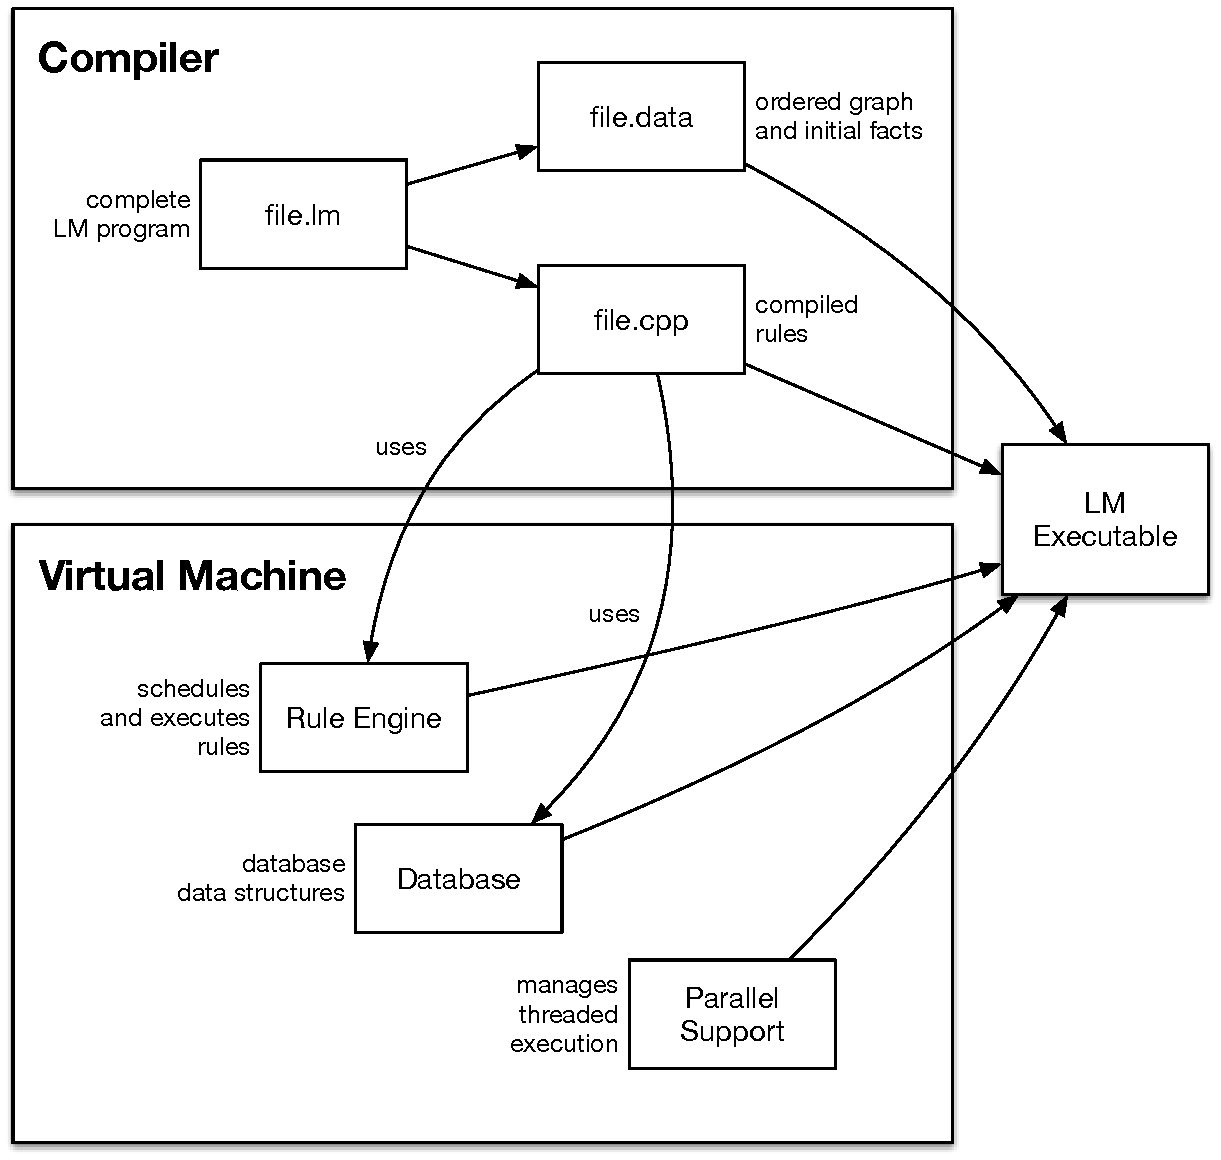
\includegraphics[width=0.7\linewidth]{figures/overview.pdf}
   \end{center}
\end{frame}

\begin{frame}[fragile]
   \frametitle{Database Structures}
   \begin{itemize}
      \item Logical fact: \texttt{prev} and \texttt{next} pointers + arguments
      \item Data structures for persistent facts:
      \begin{itemize}
         \item Tries
         \item Arrays are used for initial facts that do not need matching
      \end{itemize} 
      \item Data structures for linear facts:
      \begin{itemize}
         \item Doubly linked lists for linear facts (constant operations but linear lookup)
         \item Hash tables used for faster lookup (with dynamic or static indexing)
      \end{itemize}
   \end{itemize}
\end{frame}

\begin{frame}[fragile]
   \frametitle{Data Structures}
   \begin{itemize}
      \item Example hash table with \texttt{p(0, 20)}, \texttt{p(1, 3)},
         \texttt{p(2, 13)}, and \texttt{p(2, 43)}.
      \begin{center}
        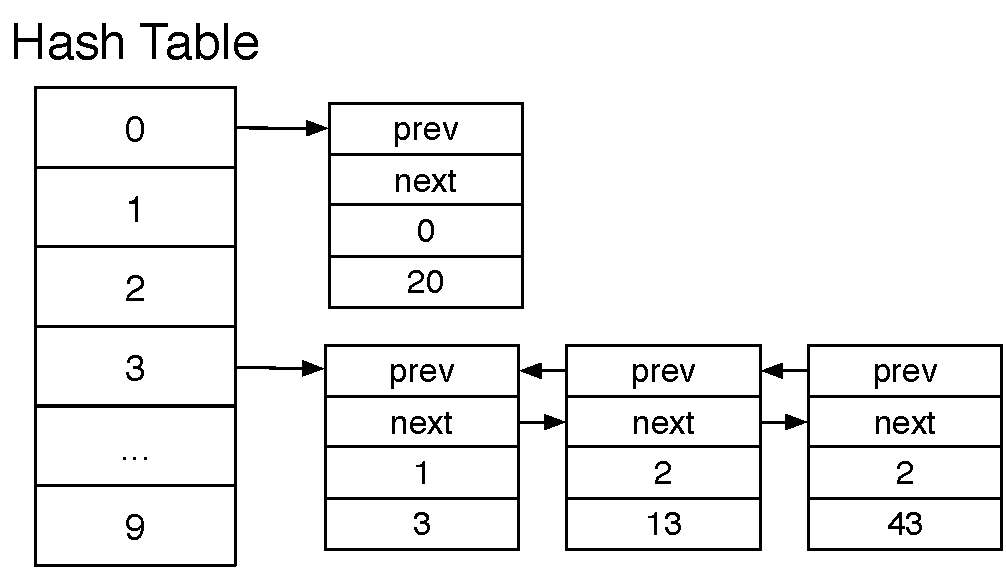
\includegraphics[width=0.7\linewidth]{hash_table.pdf}
      \end{center}
      \item Data store operations:
      \begin{itemize}
         \item Iteration (for matching)
         \item Insertion (for assertions)
         \item Deletion (for retractions)
      \end{itemize}
   \end{itemize}
\end{frame}

\subsection{Compilation Algorithm}

\begin{frame}[fragile]
   \frametitle{Compiling Rules: Iterators}
   \begin{columns}[t]
   \column{.45\textwidth}
     \begin{block}{Program}
       \begin{Verbatim}[fontsize=\tiny,commandchars=\\\{\},frame=single]
type route edge(node, node).
type linear visit(node, int).
type linear uncolored(node).
type linear colored(node, int).
type linear fail(node).

fun next(int X) : int =
   if X <> 1 then 1 else 2 end.

visit(@1, 1).
!edge(@1, @2). !edge(@1, @3).
!edge(@2, @4). !edge(@3, @4).
uncolored(A).

visit(A, P), uncolored(A)
   -o \{B | !edge(A, B) | visit(B, next(P))\},
      colored(A, P).

\alert[1]{visit(A, P), colored(A, P)}
   \alert[1]{-o colored(A, P).}
visit(A, P1), colored(A, P2), P1 <> P2
   -o fail(A).
visit(A, P), fail(A)
   -o fail(A).
\end{Verbatim}
     \end{block}
   \column{.5\textwidth}
   \begin{block}{Compiled Code}
\begin{Verbatim}[fontsize=\tiny,frame=single]
colored_list <- linked_list("colored")
visit_list <- linked_list("visit")
colored <- colored_list.head()
while(colored is valid)
{
   visit <- visit_list.head()
   while(visit is valid)
   {
      if(visit.get_int(1) == colored.get_int(1)) {
         new_colored <- create_fact("colored")
         new_colored.set_int(1, visit.get_int(1))

         colored_list.add(new_colored)

         colored <- colored_list.erase(colored)
         visit <- visit_list.erase(visit)
         goto next
      }
      visit <- visit.next()
   }
   colored <- colored.next()
next:
   continue
}
\end{Verbatim}
   \end{block}
   \end{columns}
\end{frame}

\begin{frame}[fragile]
   \frametitle{Compiling Rules: Priorities}
   \begin{columns}[t]
   \column{.45\textwidth}
     \begin{block}{Program}
       \begin{Verbatim}[fontsize=\tiny,commandchars=\\\{\},frame=single]
type route edge(node, node).
type linear visit(node, int).
type linear uncolored(node).
type linear colored(node, int).
type linear fail(node).

fun next(int X) : int =
   if X <> 1 then 1 else 2 end.

visit(@1, 1).
!edge(@1, @2). !edge(@1, @3).
!edge(@2, @4). !edge(@3, @4).
uncolored(A).

visit(A, P), uncolored(A)
   -o \{B | !edge(A, B) | visit(B, next(P))\},
      colored(A, P).

visit(A, P1), colored(A, P2), P1 <> P2
   -o fail(A).
\alert[1]{visit(A, P), colored(A, P)}
   \alert[1]{-o colored(A, P).}
visit(A, P), fail(A)
   -o fail(A).
\end{Verbatim}
     \end{block}
   \column{.5\textwidth}
   \begin{block}{Compiled Code}
\begin{Verbatim}[fontsize=\tiny,commandchars=\\\#\&,frame=single]
colored_list <- linked_list("colored")
visit_list <- linked_list("visit")
colored <- colored_list.head()
while(colored is valid)
{
   visit <- visit_list.head()
   while(visit is valid) {
      if(visit.get_int(1) == colored.get_int(1)) {
         new_colored <- create_fact("colored")
         new_colored.set_int(1, visit.get_int(1))

         colored_list.add(new_colored)

         colored <- colored_list.erase(colored)
         visit <- visit_list.erase(visit)
         \alert[1]#return&
      }
      visit <- visit.next()
   }
   colored <- colored.next()
}
\end{Verbatim}
   \end{block}
   \end{columns}
\end{frame}

\begin{frame}[fragile]
   \frametitle{Compiling Rules: Persistence Checking}
   \begin{columns}[t]
   \column{.45\textwidth}
     \begin{block}{Program}
       \begin{Verbatim}[fontsize=\tiny,commandchars=\\\{\},frame=single]
type route edge(node, node).
type linear visit(node, int).
type linear uncolored(node).
type linear colored(node, int).
type linear fail(node).

fun next(int X) : int =
   if X <> 1 then 1 else 2 end.

visit(@1, 1).
!edge(@1, @2). !edge(@1, @3).
!edge(@2, @4). !edge(@3, @4).
uncolored(A).

visit(A, P), uncolored(A)
   -o \{B | !edge(A, B) | visit(B, next(P))\},
      colored(A, P).

\alert[1]{visit(A, P), colored(A, P)}
   \alert[1]{-o colored(A, P).}
visit(A, P1), colored(A, P2), P1 <> P2
   -o fail(A).
visit(A, P), fail(A)
   -o fail(A).
\end{Verbatim}
     \end{block}
   \column{.5\textwidth}
   \begin{block}{Compiled Code}
\begin{Verbatim}[fontsize=\tiny,frame=single,commandchars=\$\#\&]
colored_list <- linked_list("colored")
visit_list <- linked_list("visit")
colored <- colored_list.head()
while(colored is valid)
{
   visit <- visit_list.head()
   while(visit is valid)
   {
      if(visit.get_int(1) == colored.get_int(1)) {
         visit <- visit_list.erase(visit)
         $textbf#goto next&
      }
      visit <- visit.next()
$textbf#next:&
      $textbf#continue&
   }
   colored <- colored.next()
}
\end{Verbatim}
   \end{block}
   \end{columns}
\end{frame}

\begin{frame}[fragile]
   \frametitle{Compiling Rules: Fact Updates}
     \begin{block}{Program}
       \begin{Verbatim}[fontsize=\tiny,commandchars=\\\{\},frame=single]
new-neighbor-pagerank(A, B, New),
neighbor-pagerank(A, B, Old)
   -o neighbor-pagerank(A, B, New).
\end{Verbatim}
\end{block}
   \begin{block}{Compiled Code}
\begin{Verbatim}[fontsize=\tiny,frame=single,commandchars=\$\#\&]
new_neighbor_pagerank_list <- linked_list("new-neighbor-pagerank")
neighbor_pagerank_table <- hash_table("neighbor-pagerank")
new_neighbor_pagerank <- new_neighbor_pagerank.head()
while(new_neighbor_pagerank is valid)
{
   neighbor_pagerank <- neighbor_pagerank_table.lookup(new_neighbor_pagerank.get_node(1))
   while(neighbor_pagerank is valid)
   {
      if(new_neighbor_pagerank.get_node(1) == neighbor_pagerank.get_node(1))
      {
         $alert[1]#neighbor_pagerank.set_float(2, new_neighbor_pagerank.get_float(2))&
         new_neighbor_pagerank <- new_neighbor_pagerank_list.erase(new_neighbor_pagerank)
         goto next
      }
      neighbor_pagerank <- neighbor_pagerank.next()
   }
   new_neighbor_pagerank <- new_neighbor_pagerank.next()
next:
   continue
}
\end{Verbatim}
   \end{block}
\end{frame}

\begin{frame}[fragile]
   \frametitle{Compiling Rules: Comprehensions}
   \begin{columns}[t]
   \column{.45\textwidth}
     \begin{block}{Program}
       \begin{Verbatim}[fontsize=\tiny,commandchars=\\\{\},frame=single]
type route edge(node, node).
type linear visit(node, int).
type linear uncolored(node).
type linear colored(node, int).
type linear fail(node).

fun next(int X) : int =
   if X <> 1 then 1 else 2 end.

visit(@1, 1).
!edge(@1, @2). !edge(@1, @3).
!edge(@2, @4). !edge(@3, @4).
uncolored(A).

\alert[1]{visit(A, P), uncolored(A)}
   \alert[1]{-o \{B | !edge(A, B) | visit(B, next(P))\},}
      \alert[1]{colored(A, P).}

visit(A, P), colored(A, P)
   -o colored(A, P).
visit(A, P1), colored(A, P2), P1 <> P2
   -o fail(A).
visit(A, P), fail(A)
   -o fail(A).
\end{Verbatim}
     \end{block}
   \column{.52\textwidth}
   \begin{block}{Compiled Code}
\begin{Verbatim}[fontsize=\tiny,frame=single,commandchars=\$\#\&]
colored_list <- linked_list("colored")
visit_list <- linked_list("visit")
uncolored_list <- linked_list("uncolored")
edge_trie <- trie("edge")
visit <- visit_list.head()
while(visit is valid)
{
   uncolored <- uncolored_list.head()
   while(uncolored is valid) {
      $alert[1]#edge <- edge_trie.first()&
      $alert[1]#while(edge is valid) {&
         $alert[1]#new_visit <- create_fact("visit")&
         $alert[1]#new_visit.set_int(1, next(visit.get_int(1)))&
         $alert[1]#send_fact(new_visit, edge.get_node(1))&
         $alert[1]#edge <- edge.next()&
      $alert[1]#}&
      new_colored <- create_fact("colored")
      new_colored.set_int(1, visit.get_int(1))
      colored_list.add(new_colored)
      visit <- visit_list.erase(visit)
      uncolored <- uncolored_list.erase(uncolored)
      goto next
   }
   uncolored <- uncolored.next()
next:
   continue
}
\end{Verbatim}
   \end{block}
   \end{columns}
\end{frame}

\begin{frame}[fragile]
   \frametitle{Compiling Rules: Aggregates}
     \begin{block}{Program}
\begin{Verbatim}[fontsize=\tiny,commandchars=\\\{\},frame=single]
update(A), pagerank(A, OldRank)
      -o [sum => V | B | neighbor-pagerank(A, B, V) | neighbor-pagerank(A, B, V)
            | pagerank(A, damping/P + (1.0 - damping) * V)].
\end{Verbatim}
\end{block}
   \begin{block}{Compiled Code}
\begin{Verbatim}[fontsize=\tiny,frame=single,commandchars=\$\#\&]
pagerank_list <- linked_list("pagerank")
update_list <- linked_list("update")
neighbor_pagerank_list <- linked_list("neighbor_pagerank_list")
pagerank <- pagerank_list.head()
while(pagerank is valid) {
   update <- update_list.head()
   while(update is valid) {
      $alert[1]#V <- 0.0&
      $alert[1]#neighbor_pagerank <- neighbor_pagerank_list.head()&
      $alert[1]#while(neighbor_pagerank is valid) {&
         $alert[1]#V <- V + neighbor_pagerank.get_float(2)&
         $alert[1]#neighbor_pagerank <- neighbor_pagerank.next()&
      $alert[1]#}&
      pagerank.set_float(1, damping / P + (1.0 - damping) * V)
      update <- update_list.erase(update)
      goto next
   }
   pagerank <- pagerank.next()
next:
   continue
}
\end{Verbatim}
   \end{block}
\end{frame}
\section{Experimental Results}

\begin{frame}
   \frametitle{Experimental Setup}
   \begin{itemize}
      \item Compare LM against hand-written C/C++ programs
      \item Using the following programs:
      \begin{itemize}
         \item Shortest Path: compute shortest distance from some nodes to all nodes.
         \item N-Queens: puzzle.
         \item Belief Propagation: de-noise an image.
         \item Heat Transfer: transfer heat in a graph.
         \item MiniMax: AI algorithm.
      \end{itemize}
   \end{itemize}
\end{frame}

\frame
{
   \frametitle{Absolute Runtime}
\begin{center}
\scalebox{0.7}{
    \begin{tabular}{c || c | c | c | c}
    \textbf{Program} & \textbf{Size} & \textbf{C Time} (s) & \textbf{LM} 
    & \textbf{Other} \\ \hline \hline
    \multirow{3}{*}{Shortest Path} & US Airports & 0.1 & 3.9 & 13.3 (python) \\
                                   & OCLinks & 0.4 & 5.6 & 11.2 (python) \\
                                   & Powergrid & 0.9 & 3.5 & 10.6 (python) \\
                                   & Email & 10.98 & 1.7 & 12.20 (python) \\
                                   \hline

    \multirow{4}{*}{N-Queens} & 11 & 0.2 & 1.4 & 20.8 (python) \\
                              & 12 & 1.3 & 3.2 & 24.1 (python) \\
                              & 13 & 7.8 & 3.8 & 26.0 (python) \\
                              & 14 & 49 & 4.5 & 28.0 (python) \\ \hline
    \multirow{4}{*}{Belief Propagation} & 50 & 2.8 & 1.3 & 1.1 (GL) \\
                                        & 200 & 51 & 1.3 & 1.1 (GL) \\
                                        & 300 & 141 & 1.3 & 1.1 (GL) \\
                                        & 400 & 180 & 1.3 & 1.1 (GL) \\
                                        \hline
    \multirow{2}{*}{Heat Transfer} & 80 & 7.3 & 4.6 & - \\
                                   & 120 & 32 & 5.3 & - \\ \hline

  MiniMax & - & 7.3 & 3.2 & 9.3 (python) \\
    \end{tabular}
}
\end{center}
}

\frame
{
   \frametitle{Scalability}
   \begin{center}
      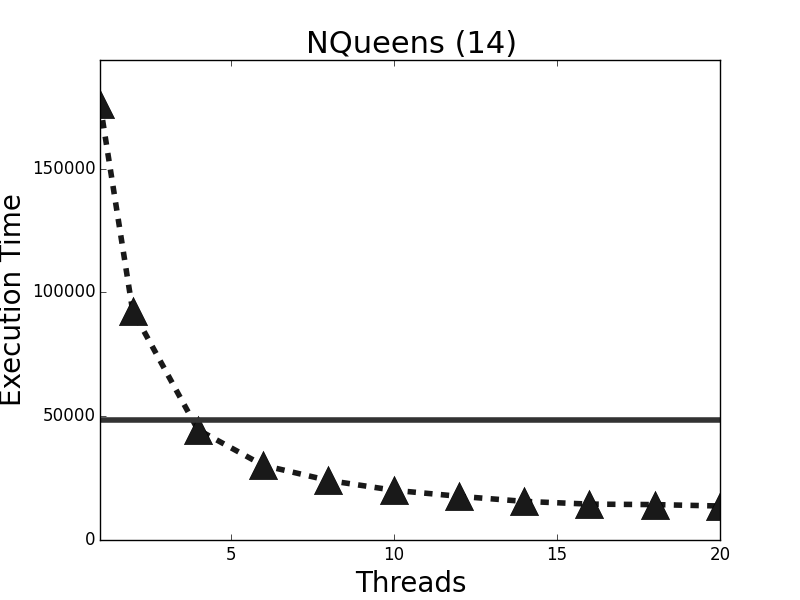
\includegraphics[width=0.5\linewidth]{figures/scale-8queens-14.png}
      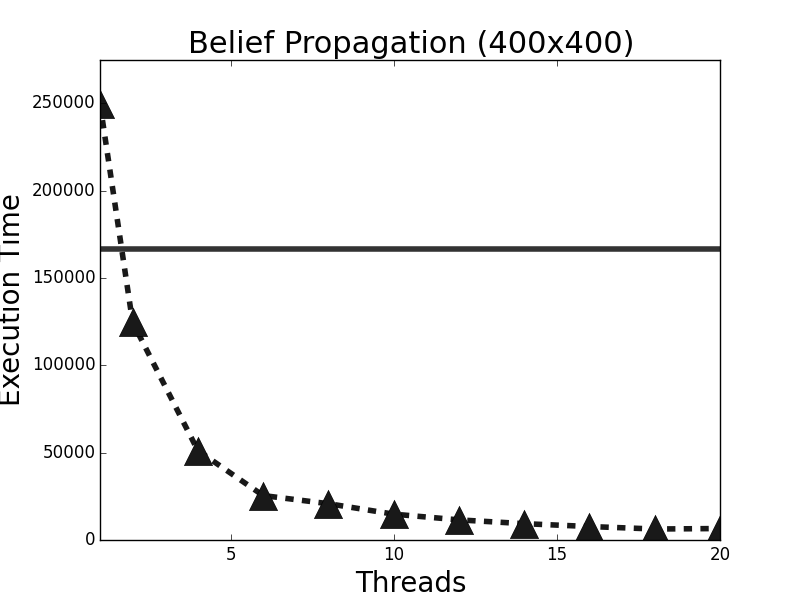
\includegraphics[width=0.5\linewidth]{figures/scale-belief-propagation-400.png}
   \end{center}
}

\begin{frame}
   \frametitle{Conclusions}
   \begin{itemize}
      \item New compilation algorithm that turns logical rules into C++ code

      \begin{itemize}
         \item Support for rule priorities, comprehensions and aggregates
         \item Detection of fact updates and persistent linear updates
         \item However, memory layout often matters more than the
               compilation algorithms!
      \end{itemize}

      \item Decent results show that it is possible to run LM programs that are
         at most one order of magnitude slower than corresponding C programs

      \begin{itemize}
         \item With parallelism it becomes possible to run faster than C
      \end{itemize}

      \item Future work: uniqueness analysis, fact invariants, better memory
         layout, custom data structures
      \begin{itemize}
         \item Recover the \emph{imperativeness} of linear logic programs
      \end{itemize}
   \end{itemize}
\end{frame}


\begin{frame}{Thank You}
\begin{center}
{\Huge Thank you for your time!}
\end{center}
\end{frame}

\end{document}

